% !TeX root = ../main.tex
\chapter{The CD4AI Pattern}
\label{chap:cd4ai}

CD4AI is a continuous delivery pattern that addresses the following problem:
\enquote{How can teams turn failures observed during the use of AI-enabled
systems into evaluation cases that support subsequent changes?}
This chapter presents the pattern and its feedback loop.
Chapter~\ref{chap:case-studies} examines how its stages appear in selected
systems and documented workflows.

\section{Context, Problem, and Intent}
\label{sec:cd4ai-context}

% Context

Foundation models are trained on broad data at scale and can be adapted to
a range of downstream tasks~\cite{Bommasani:FoundationModels:2021}.
Applications built around language foundation models can change their behavior
through modifications to prompts, retrieved context, tools, and orchestration,
without necessarily retraining the underlying
model~\cite{Schluntz:BuildingEffectiveAgents:2024}.
By avoiding a model-training cycle for such changes, application teams can
shorten the implementation cycle and introduce behavioral changes within their
ordinary software development workflow.

In this setting, evaluating AI-dependent behavior becomes part of the
application team's delivery responsibilities, even when the team does not
develop or train the underlying model. A change that is quick to implement
may still require substantial evaluation. The resulting challenge is to assess
its effects on established behavior while incorporating failures discovered
during use into future evaluations.

% Optional motivation: add a concrete observation from the startup experience,
% distinguishing personal observations from claims about development practices
% in general. Keep implementation details for the relevant case study.

% Problem

Initial evaluations cannot be assumed to cover every interaction that will
emerge during use. Teams therefore need a process for identifying candidate
failures, reviewing them, and turning confirmed defects into useful evaluation
cases. Collecting interactions alone does not establish this connection: the
cases must capture expected behavior and return to the evaluation suite used
to assess subsequent changes.

A further difficulty arises when a suite contains both known unresolved
limitations and behavior that the team expects to preserve. An undifferentiated
failure report does not establish whether a proposed change introduced a
regression or whether a known limitation persists. The evaluation process must
retain enough context to interpret the result and support a delivery decision.

% Intent

CD4AI aims to support frequent delivery while preserving established behavior
by connecting evaluation, monitoring, and curation in a recurring feedback loop.
Although applications built around language foundation models motivate the
discussion here, the pattern is described in terms of these responsibilities,
rather than a particular model or evaluation framework. Its intent is to make
observed failures inform future validation, without guaranteeing that every
failure will be discovered or that a previously observed defect will never recur.

Following the terminology in Section~\ref{sec:background-evaluation}, these
cases can document unresolved limitations, support confirmation of fixes, and
help detect regressions. The evaluation stage includes these purposes;
creating a case does not imply that the corresponding defect has been fixed.

\section{Overview of the Feedback Loop}
\label{sec:cd4ai-overview}

CD4AI maintains an evolving evaluation suite informed by observed application
behavior. Selected interactions are reviewed to establish expected behavior
and prepare reusable cases. These cases are exercised against subsequent
application versions, and the results inform development and delivery
decisions. The pattern assigns three responsibilities:

\begin{description}
  \item[Evaluation.] Exercise application versions against retained cases and
    interpret the results as evidence about capabilities, unresolved
    limitations, and changes in established behavior.
  \item[Monitoring.] Collect interactions during use and identify behavior
    worth investigating, producing candidates for review.
  \item[Curation.] Review selected interactions, determine the desired behavior,
    and prepare reusable evaluation cases with explicit assessment criteria.
\end{description}

Figure~\ref{fig:cd4ai-feedback-loop} summarizes the transitions between these
stages and the return of curated cases to evaluation.

\begin{figure}[htbp]
  \centering
  % Included inside a figure environment in Chapter 4.
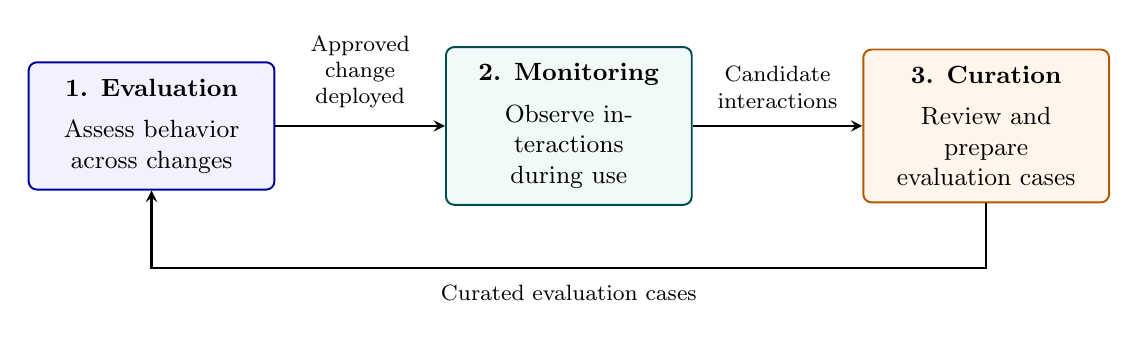
\begin{tikzpicture}[
  stage/.style={
    draw, rounded corners=3pt, line width=0.7pt,
    text width=2.7cm, minimum height=1.5cm,
    inner sep=6pt, align=center, font=\small
  },
  flow/.style={->, >=stealth, line width=0.8pt},
  transition/.style={align=center, font=\footnotesize, fill=white, inner sep=3pt}
]
  \node[stage, draw=blue!60!black, fill=blue!5] (testing) at (0,0)
    {\textbf{1. Evaluation}\\[4pt]Assess behavior\\across changes};
  \node[stage, draw=teal!60!black, fill=teal!5] (monitoring) at (5.3,0)
    {\textbf{2. Monitoring}\\[4pt]Observe interactions\\during use};
  \node[stage, draw=orange!70!black, fill=orange!8] (curation) at (10.6,0)
    {\textbf{3. Curation}\\[4pt]Review and prepare\\evaluation cases};

  \draw[flow] (testing.east) -- node[transition, above=3pt]
    {Approved\\change\\deployed} (monitoring.west);
  \draw[flow] (monitoring.east) -- node[transition, above=3pt]
    {Candidate\\interactions} (curation.west);
  \draw[flow] (curation.south) -- (10.6,-1.8)
    -- node[transition, below=3pt] {Curated evaluation cases}
    (0,-1.8) -- (testing.south);
\end{tikzpicture}

  \caption{The CD4AI feedback loop. Evaluation provides evidence for delivery
    decisions; monitoring supplies candidate interactions for review;
    curation prepares evaluation cases for subsequent assessments.}
  \label{fig:cd4ai-feedback-loop}
\end{figure}

Application changes, including defect fixes, are implemented through the team's
development process and assessed in the evaluation stage. Curation specifies cases
and expected behavior; it does not itself repair the application. The diagram
summarizes the flow of evaluation evidence rather than every development activity.

The connections between stages are essential. A stored interaction must become
a case that can be exercised and assessed; the retained case must participate
in subsequent evaluations; and the results must inform a development or
delivery decision. Collecting logs or creating a dataset without these
connections does not establish the feedback loop.

The pattern distinguishes three decisions: what evidence to retain, how to
interpret evaluation results, and what action those results warrant. Retaining
a case does not imply that its expected behavior has already been achieved,
and observing a failure does not by itself identify a new regression. An
explicit acceptance policy determines which results block delivery.

\noindent\emph{Working refinement.} The distinction between known limitations
and deterioration in established behavior is proposed here as a responsibility
of result interpretation. Chapter~\ref{chap:case-studies} will examine the
extent to which each documented workflow supports it, separately from the
evidence for the three-stage feedback loop itself.

\subsection{Following a Failure through the Cycle}
\label{sec:cd4ai-dynamics}

Consider a hypothetical assistant that gives an incorrect answer about product
eligibility. Monitoring retains the interaction and flags it for review.
During curation, a reviewer confirms the defect, identifies the relevant policy,
and prepares a case describing the input, necessary context, and expected
behavior. The case is retained even if the team cannot immediately fix the
application. Its evaluation result makes the unresolved limitation visible.

When a developer proposes a change, the case helps assess whether the desired
behavior has been achieved. Other retained cases help assess the effects on
previously established behavior. If the fix is confirmed under the team's
evaluation criteria, the case can then be used to protect that behavior during
later changes. A subsequent failure calls for investigation of a possible
regression, taking execution and assessment variability into account.

This example illustrates the proposed process rather than an observed result.
The same retained case supports different evaluation purposes over time;
the process does not require separate copies of it for each purpose.

\section{Evaluation}
\label{sec:cd4ai-testing}

\subsection{Evaluation Cases and Expected Behavior}
\begin{itemize}
  \item Explain how cases prepared for expected behavior complement cases
    derived from previously observed failures, including unresolved defects
    and cases retained for regression protection.
  \item Describe the input, relevant context, expected behavior, and evaluation
    criterion needed to make a retained case useful.
\end{itemize}

\subsection{Evaluation Criteria and Variability}
\begin{itemize}
  \item Clarify how tests and evaluations are used in this chapter, drawing on
    the terminology introduced in Section~\ref{sec:background-evaluation}.
  \item Discuss possible checks and evaluators, including their limitations when
    several outputs are acceptable or responses vary between runs.
\end{itemize}

\subsection{Interpreting Results across Changes}
\label{sec:cd4ai-result-interpretation}

A case documenting an unresolved defect can guide improvement; exercising it
against a proposed fix supports confirmation; retaining it after the behavior
is established supports regression protection. These are evaluation purposes,
not necessarily different data structures or mutually exclusive categories.
As discussed in Section~\ref{sec:background-evaluation-purpose}, the purpose
of a case cannot be inferred solely from whether it currently passes or fails.

Interpreting a result requires the expected behavior, the application version
assessed, and the relevant reference evidence. That evidence may include a
reviewed record of the unresolved defect, results from an accepted baseline,
or explicit requirements for behavior that must be preserved. A continuing
failure should remain visible as a limitation; a change from previously
acceptable behavior should be investigated as potential deterioration.
Scores may also worsen while remaining below a pass threshold, so a comparison
should not rely exclusively on binary verdicts.

Where results are compared across versions, the cases, assessment criteria,
and execution conditions must support a meaningful comparison. New cases
without reference results and unsuccessful evaluation executions should be
identified separately. The implementation must also account for variability
in the application and its evaluators before attributing a difference to the
proposed change.

\subsection{Integration with the Delivery Pipeline}

The acceptance policy specifies how evaluation evidence affects delivery.
A critical unmet requirement may block release even when the defect is already
known. Other unresolved limitations may be reported separately under an explicit
decision to defer their resolution. Such a decision does not change the expected
behavior or establish that the defect has been fixed.

The pattern leaves the organization and enforcement mechanisms to the
implementation. Teams may use separate suites, metadata, or filtered views to
distinguish evaluation purposes. They may apply absolute requirements,
comparisons against an accepted baseline, or both. Likewise, some evaluations
may block delivery while others inform improvement work. The shared
responsibility is to make the interpretation and resulting decision explicit;
exactly two datasets or a universal numerical threshold are not requirements.

\section{Monitoring}
\label{sec:cd4ai-monitoring}

\subsection{Observing Interactions}
\begin{itemize}
  \item Describe what information can help reconstruct behavior during use:
    inputs, outputs, retrieved context, tool calls, and user feedback.
  \item Explain how the available observations constrain subsequent review.
\end{itemize}

\subsection{Selecting Candidates for Review}
\begin{itemize}
  \item Describe candidate signals, such as negative feedback, unexpected tool
    behavior, and guardrail violations, alongside sampling of interactions.
  \item Explain the trade-off between broad discovery and review effort, and
    distinguish a suspected failure from a confirmed defect.
\end{itemize}

\section{Curation}
\label{sec:cd4ai-curation}

\subsection{Reviewing Candidate Interactions}
\begin{itemize}
  \item Explain how human review, AI-assisted review, or a combination can assess
    selected interactions and distinguish defects from noise.
  \item Describe the role of expected behavior and review rationales; discuss
    uncertain judgments and evaluator limitations.
\end{itemize}

\subsection{Preparing Evaluation Cases}
\begin{itemize}
  \item Explain how a confirmed defect becomes a reusable input or scenario with
    an expected behavior and an evaluation criterion.
  \item Discuss which context must be retained and how cases are selected and
    maintained as the suite grows.
\end{itemize}

\subsection{Returning Cases to Evaluation}
\begin{itemize}
  \item Make the handoff explicit: recording a review does not by itself add a
    case to the evaluation suite.
  \item Describe manual and automated ways to retain the case, evaluate a fix,
    and check subsequent changes.
  \item Explain how the case remains linked to its originating observation,
    review, expected behavior, and known defect status so that later results
    can be interpreted.
\end{itemize}

\section{Forces}
\label{sec:cd4ai-forces}

\noindent\emph{Working formulation: the following forces will be revisited
as the case studies are developed.}

Testability, robustness, and evolvability are desired qualities that can
reinforce one another. Testability helps teams assess whether a proposed change
preserves expected behavior before deployment. Robustness concerns the
application's ability to maintain acceptable behavior under varying conditions,
while evolvability concerns its ability to accommodate change. The evaluation
suite must also evolve to remain useful as the application changes.

These qualities need not oppose one another in every pairwise comparison.
The forces considered here instead express tensions between desired outcomes
and the constraints on achieving them. The pattern aims to address three
such tensions:

\begin{itemize}
  \item \textbf{Confidence in changes and delivery speed:} teams need evidence
    that changes preserve expected behavior, but running more extensive
    evaluations requires execution time and maintenance effort. The validation
    process must fit the time and resources available for frequent delivery.
  \item \textbf{Failure discovery and review capacity:} teams need to discover
    failures beyond those covered by existing tests, but collecting more
    candidate interactions increases the curation workload. Broad discovery
    must be balanced with the capacity to review candidates and prepare useful
    evaluation cases.
  \item \textbf{Behavior preservation and adaptation:} historical regression
    cases help check established behavior, but changing requirements can make
    some expectations outdated. Teams must distinguish unintended regressions
    from intended changes and maintain the suite accordingly.
\end{itemize}

Evaluation, monitoring, and curation work together to address these tensions.
Evaluation supplies evidence about proposed changes, monitoring supplies
interactions for investigation, and curation determines which interactions
should become evaluation cases and what behavior those cases should check.
The cycle does not remove the costs or trade-offs; its implementation must
establish how these responsibilities fit the team's delivery process.

% Writing notes:
% Keep the desired qualities distinct from the concrete tensions above.
% Do not claim that greater testability necessarily lowers robustness or
% evolvability. Better testing can support both.
% Validate this working formulation against Chapter 5: look for evidence of
% evaluation cost, candidate selection, review workload, and changes to expected
% behavior. Do not present these as findings before examining the evidence.
% Explain how the stages address the tensions without forcing a one-to-one
% correspondence between a stage and a force. Connected paragraphs are enough;
% pairwise-comparison subsections are not necessary.
% Pattern-writing guidance discussed during review:
% https://www.hillside.net/index.php/a-pattern-language-for-pattern-writing
% Add a formal citation if this guidance is used in the final argument.

\section{Consequences and Limitations}
\label{sec:cd4ai-consequences}

\begin{itemize}
  \item Discuss the intended benefit of an evaluation suite informed by actual
    use, separating expected benefits from measured outcomes.
  \item Discuss the costs of observation, review, and maintaining and running
    the growing suite.
  \item Explain limits arising from unobserved interactions, missed signals,
    reviewer errors, and variable behavior. Avoid guarantees of complete
    coverage or prevention of every recurrence.
  \item Introduce the case studies as an examination of how these responsibilities
    and connections appear in different systems and workflows.
\end{itemize}
